\documentclass[twocolumn]{article}
\usepackage[top=15mm,bottom=15mm,left=15mm,right=15mm]{geometry}
\usepackage{amsmath,amssymb}
\usepackage{titlesec}
\usepackage{setspace}
\usepackage[dvipdfmx]{graphicx}
\usepackage{caption}
\setstretch{1.0}
\setlength{\parindent}{0pt}
\setlength{\parskip}{0pt}
\setlength{\abovedisplayskip}{3pt}
\setlength{\belowdisplayskip}{3pt}
\setlength{\abovedisplayshortskip}{3pt}
\setlength{\belowdisplayshortskip}{3pt}
\titlespacing*{\section}{0pt}{10pt}{5pt}
\titlespacing*{\subsection}{0pt}{8pt}{4pt}
\pagestyle{empty}

\begin{document}

\begin{enumerate}
  \item (a)の回路における電力の導出
    \begin{align*}
    &\text{入力電圧の最大値を} E_m \text{とすると}\\
    e     &= E_m \sin \omega t \\ 
    i     &= \frac{e}{R} = \frac{E_m}{R} \sin \omega t \\ 
    ei    &= E_m \sin \omega t \cdot \frac{E_m}{R} \sin \omega t \\ 
          &= \frac{E_m^2}{R} \sin^2 \omega t \\ 
          &= \frac{E_m^2}{R} \left( 1 - \cos 2 \omega t \right) \\ 
    E     &= \frac{E_m}{\sqrt{2}} \text{より,} \\ 
    E_m^2 &= 2E^2 \text{であるから,} \\ 
    ei    &= ei_R = \frac{E^2}{R} \left( 1 - \cos 2 \omega t \right) \\
    \end{align*}

  \item (b)の回路における電力の導出
    \begin{align*}
    e &= \sqrt{2}E \sin \omega t \\ 
    &\text{インダクタンス } L\,[\text{H}] \text{ に流れる電流を } i\,[\text{A}] \\
    &\text{とすると,誘導起電力 } e_L\,[\text{V}] \text{ は} \\
    e_L &= -L \frac{di}{dt} \\
    &e + e_L = 0 \text{ が成り立つため,} \\
    e &= L \frac{di}{dt} \\ 
    \frac{e}{L} dt &= di \\ 
    \int di &= \int \frac{e}{L} dt \\ 
    i &= \int \left(\sqrt{2} E \sin \omega t dt\right) \\ 
      &= - \sqrt{2} \frac{E}{\omega L} \cos \omega t \\ 
      &= \sqrt{2}\frac{E}{\omega L}\sin \left(\omega t - \frac{\pi}{2}\right) \\ 
    ei  &= \frac{2E^2}{\omega L}\sin \omega t \cdot \sin \left(\omega t - \frac{\pi}{2}\right) \\
    &\text{積和の公式} \\
    &\sin\alpha \sin \beta = -\frac{1}{2} \left( \cos \left(\alpha + \beta\right) - \cos \left(\alpha - \beta\right) \right)\\
    &\text{を用いて変形すると}\\
    ei  &= \frac{2E^2}{\omega L} \left(- \frac{1}{2} \left(\cos\left(\omega t + \omega t - \frac{\pi}{2}\right) \right. \right. \\
        &  \qquad\left.\left. - \cos\left(\omega t - \omega t + \frac{\pi}{2}\right) 
        \right) \right)\\
        &= -\frac{E^2}{\omega L} \cos \left(2\omega t - \frac{\pi}{2}\right) 
    \end{align*}

  \item (c)の回路における電力の導出
    \begin{align*}
    e &=\sqrt{2}E\sin\omega t\\
    &\text{静電容量} C\,[\text{F}] \text{ に加わる電圧を } v\,[\text{V}] \\
    &\text{とすると,流れる電流 } i\,[\text{A}] \text{ は} \\
    i   &= \frac{dq}{dt} = \frac{d}{dt}Cv \\
        &= C \frac{d \left(\sqrt{2}E\sin \omega t\right)}{dt} \\
        &= \sqrt{2}\omega CE\cos\omega t\\
    &\text{これらから,電力eiは}\\
    ei &= 2E^2 \omega C \sin\omega t \cos \omega t \\ 
    &= E^2 \omega C \sin \left(2 \omega t\right)\\
    \end{align*}

    \begin{center}
      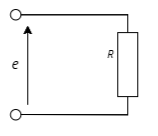
\includegraphics[width=0.6\linewidth]{./Circuits/Circuits_a.png}
      \captionof{figure}{回路a} % ✅ OK
    \end{center}
    \begin{center}
      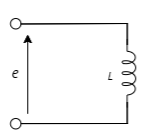
\includegraphics[width=0.6\linewidth]{./Circuits/Circuits_b.png}
      \captionof{figure}{回路b} % ✅ OK
    \end{center}
    \begin{center}
      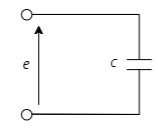
\includegraphics[width=0.6\linewidth]{./Circuits/Circuits_c.png}
      \captionof{figure}{回路c} % ✅ OK
    \end{center}

    \item (d)の回路における電力の導出
    \begin{align*}
      e   &=\sqrt{2}E\sin\omega t\\
      &\text{また,各素子の電圧降下の合成と考えると}\\
      e   &=iR + L \frac{di}{dt} \text{とも表すことができる.} \\
      &\text{抵抗とインダクタンスの合成インピーダンスを} Z \text{,}\\
      &\text{合成インピーダンスの位相のずれを} \Phi \text{とすると}\\
      &\text{電流} i \text{は,}\\
      i   &= \frac{\sqrt{2}E}{\|Z\|} \sin \left( \omega t - \Phi\right)\\
      &\text{この} i \text{を用いて電力} ei \text{を表すと,}\\
      ei  &= \sqrt{2}E\sin\omega t \cdot \frac{\sqrt{2}E}{\|Z\|} \sin \left( \omega t - \Phi\right) \\
          &= \frac{2E^2}{\|Z\|}\sin\omega t \sin \left(\omega t - \Phi\right)\\
      &\text{加法定理を用いて,}\sin \left(\omega t - \Phi\right) \text{を変形すると}\\
      ei  &= \frac{2E^2}{\|Z\|}\sin\omega t \left(\sin\omega t \cos \Phi - \cos\omega t \sin \Phi\right)\\
          &= \frac{2E^2}{\|Z\|} \left(\sin^2 \omega t \cos \Phi - \sin\omega t \cos\omega t \sin \Phi\right)\\
          &= \frac{2E^2}{\|Z\|} \left(\sin^2 \omega t \cos \Phi \right) - \frac{2E^2}{\|Z\|} \left(\sin\omega t \cos\omega t \sin \Phi\right)\\
      &\text{左の項にはsinの半角公式}\\
      &\text{右の項には} \sin \alpha \cos \beta \text{の積和公式を用いて変形すると}\\
      ei  &= \frac{2E^2}{\|Z\|} \left(\left(\frac{1-\cos2\omega t}{2}\right)\cos \Phi\right)\\
          &- \frac{2E^2}{\|Z\|}\left(\frac{1}{2}\left(\sin2\omega t + \sin0\right) \sin \Phi\right)\\
          &= \frac{E^2}{\|Z\|} \cos \Phi \left(1-\cos2\omega t\right) - \frac{E^2}{\|Z\|} \sin \Phi\sin2\omega t \\
      &\text{また,各素子における電力を求める.}\\
          &\text{抵抗での電圧降下}e_R \text{は,}\\
          e_R &= iR = \frac{\sqrt{2}E}{\|Z\|} R \sin \left( \omega t - \Phi\right)\\
          &\text{であるから,}\\
          ei_R&= \frac{\sqrt{2}E}{\|Z\|} R \sin \left( \omega t - \Phi\right) \cdot \frac{\sqrt{2}E}{\|Z\|} \sin \left( \omega t - \Phi\right)\\
              &= \frac{2E^2}{\|Z\|^2} R \sin^2 \left(\omega t - \Phi\right)\\
          &\text{半角の公式を用いて}\\
          &= \frac{2E^2}{\|Z\|^2} R \left( \frac{1-\cos2\left(\omega t - \Phi\right)}{2} \right)\\
          &= \frac{E^2}{\|Z\|^2} R \left( 1-\cos2\left(\omega t - \Phi\right)\right)\\
          &R\text{と}\omega L \text{との位相差は} \frac{\pi}{2} \text{であり,}\\
          &\text{合成インピーダンス}Z\text{の位相差を}\Phi \text{とすると,}\\
    \end{align*}
    \begin{align*}
      &\frac{R}{\|Z\|} = \cos \Phi \text{となるため,}\\
      ei_R&= \frac{E^2}{\|Z\|} \cos \Phi \left( 1-\cos2\left(\omega t - \Phi\right)\right)\\
      &\text{次にコイルでの電圧降下}e_L \text{は,}\\
      e_L &= L \frac{di}{dt} = L \frac{d}{dt} \left( \frac{\sqrt{2}E}{\|Z\|} \sin \left( \omega t - \Phi\right) \right)\\
          &= \frac{\sqrt{2}E}{\|Z\|} \omega L \cos \left(\omega t - \Phi\right)\\
      &\text{であるから,}\\
      ei_L&= \frac{\sqrt{2}E}{\|Z\|}\omega L \cos\left(\omega t - \Phi\right) \cdot \frac{\sqrt{2}E}{\|Z\|} \sin \left( \omega t - \Phi\right)\\
          &= \frac{2E^2}{\|Z\|^2} \omega L \cos\left(\omega t - \Phi\right)\sin\left(\omega t - \Phi\right)\\
      &\text{積を和に直す公式を用いて変形すると,}\\
      ei_L&= \frac{2E^2}{\|Z\|^2}\omega L \left(\frac{1}{2} \left(\sin 2\omega t - 2\Phi\right)\right) \\
          &= \frac{E^2}{\|Z\|^2}\omega L \left(\sin 2\omega t - 2\Phi\right)\\
      &\text{また,} \frac{\omega L}{\|Z\|} = \sin \Phi \text{となるため,}\\
      ei_L&= \frac{E^2}{\|Z\|}\sin \Phi \left(\sin 2\omega t - 2\Phi\right)\\
    \end{align*}

    \begin{center}
      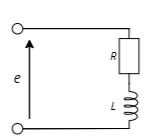
\includegraphics[width=0.6\linewidth]{./Circuits/Circuits_d.png}
      \captionof{figure}{回路d} % ✅ OK
    \end{center}

    \item (e)の回路における電力の導出
    \begin{align*}
      e   &=\sqrt{2}E\sin\omega t\\
      &\text{並列接続であるから,抵抗および}\\
      &\text{インダクタンスにかかる電圧は等しいので,}\\
      e   &= e_R = e_L\\
      &\text{また,各素子における電圧降下で考えると,}\\
      e   &= {i_R}R = L\frac{di_L}{dt}\\
    \end{align*}
    
    \begin{align*}      
      &\text{抵抗に流れる電流は,オームの法則より,}\\
      i_R &= \frac{e}{R}\\
          &= \frac{\sqrt{2}E}{R}\sin \omega t\\
      &\text{インダクタンスに流れる電流は,}\\
      e   &= L\frac{di_L}{dt}\\
      \frac{e}{L}dt &= di_L\\
      \int di_L &= \int \frac{e}{L}dt\\
      i_L &= \frac{\sqrt{2}E}{L} \int \sin \omega t dt\\
          &= -\frac{\sqrt{2}E}{\omega L} \cos \omega t\\
      &\text{ところで,合成アドミタンス}Y\text{は,}\\
      Y   &= \frac{1}{R} + \frac{1}{j\omega L}\\
          &= \frac{1}{R} - j\frac{1}{\omega L}\\
      \|Y\| &= \sqrt{{\left(\frac{1}{R}\right)}^2 + {\left(\frac{1}{\omega L}\right)}^2}\\
      &\text{つまり,合成インピーダンス}Z\text{は,}\\
      \|Z\| &= \frac{\omega LR}{\sqrt{R^2 + {\left(\omega L\right)}^2}}\\
      &\text{電圧を基準として電流の位相差をを考えると,}\\
      &\text{電圧と同位相である}\frac{1}{R}\text{と,}-\frac{\pi}{2}\text{ずれている}\frac{1}{\omega L}\\
      &\text{によって得られる電流は}Y\text{の位相であるため,}\\
      &\text{Yの位相を}\Phi\text{とすると,}\\
      &\cos \Phi = \frac{\frac{1}{R}}{\|Y\|} = \frac{\|Z\|}{R} \Rightarrow  \frac{1}{R} = \frac{\cos \Phi}{\|Z\|}\\
      &\sin \Phi = \frac{\frac{1}{\omega L}}{\|Y\|} = \frac{\|Z\|}{\omega L} \Rightarrow  \frac{1}{\omega L} = \frac{\sin \Phi}{\|Z\|}\\
      &\text{となる.これらから電流}i_R\text{と,}i_L\text{を変形すると,}\\
      i_R   &= \frac{\sqrt{2}E}{R}\sin \omega t\\
            &= \frac{\sqrt{2}E}{\|Z\|}\cos \Phi \sin \omega t\\
      i_L   &= -\frac{\sqrt{2}E}{\omega L} \cos \omega t\\
            &= -\frac{\sqrt{2}E}{\|Z\|} \sin \Phi \cos \omega t\\
      &\text{となり,式3.17,式3.18が得られ,各素子の電力は,}\\
    \end{align*}
    \begin{align*}
      ei_R  &= \sqrt{2}E\sin\omega t \cdot \frac{\sqrt{2}E}{\|Z\|}\cos\Phi\sin\omega t\\
            &= \frac{2E^2}{\|Z\|}\cos\Phi\sin^2\omega t\\
      &\text{半角の公式を用いて,}\\
            &= \frac{2E^2}{\|Z\|}\cos\Phi\left(\frac{1 - \cos 2\omega t}{2}\right)\\
            &= \frac{E^2}{\|Z\|}\cos\Phi\left(1 - \cos 2\omega t\right)\\
      ei_L  &= \sqrt{2}E\sin\omega t \cdot \left(-\frac{\sqrt{2}E}{\|Z\|} \sin \Phi \cos \omega t \right)\\
            &= \frac{2E^2}{\|Z\|} \sin\Phi \sin\omega t\cos\omega t \\
      &\text{積和の公式を用いて,}\\
      &= \frac{2E^2}{\|Z\|}\sin\Phi \left( \frac{1}{2} \left(\sin 2\omega t - \sin 0 \right) \right)\\
      &= \frac{E^2}{\|Z\|}\sin\Phi\sin 2\omega t\\
      \therefore ei_R  &= \frac{E^2}{\|Z\|}\cos\Phi\left(1 - \cos 2\omega t\right)\\
      \therefore ei_L  &= \frac{E^2}{\|Z\|}\sin\Phi\sin 2\omega t\\
    \end{align*}

    \item (f)の回路における電力の導出
    \begin{align*}
      e &= \sqrt{2}E\sin\omega t\\
      &\text{ここで,各素子の合成インピーダンスを考える.}\\
      Z_{R1} &= R_1\\
      Z_{RL} &= R_2 + j\omega L\\
      &\text{であるから,並列接続部分の合成インピーダンスは,}\\
      \frac{1}{Z_p} &= \frac{1}{Z_{R1}} + \frac{1}{Z_{RL}}\\
      &\text{回路全体の合成インピーダンスを}Z\text{とすると,}\\
      Z     &= R_0 + Z_p\\
      &Z\text{の位相を}\Phi\text{とすると,回路に流れる電流}i_s\text{は,}\\
      i_s   &= \frac{\sqrt{2}E}{\|Z\|}\sin\left(\omega t - \Phi\right)\\
      &\text{となり,電力は}\\
      ei    &= \sqrt{2}E\sin\omega t \cdot \frac{\sqrt{2}E}{\|Z\|}\sin\left(\omega t - \Phi\right) \\
            &= \frac{E^2}{\|Z\|} \cos \Phi \left(1-\cos2\omega t\right) - \frac{E^2}{\|Z\|} \sin \Phi\sin2\omega t \\
      &\text{また,各素子の電力は,その素子に流れる電流,}\\
      &\text{その素子にかかる電圧,その素子のインピーダンスに}\\
      &\text{よって立式されている.}\\
    \end{align*}

\end{enumerate}

\end{document}
